%======================================================================
% L09_SF_Liouville_microcanon_annotated.pdf
%======================================================================
\section{Statistický popis makro-systémů}
\strana{L09-1}

\begin{minipage}[t]{0.6\textwidth}
\begin{enumerate}[label=\arabic*)]
  \item \underline{mikrostav $\mu$:}
  \begin{itemize}
    \item[$\to$] $H = H\big(\{p_i,q_i\}_{i=1}^{3N}\big)$ + fázový prostor = systém
    \item[$\to$] stav: hodnoty $\forall\, p_i, q_i$
    \item[$\to$] vývoj systému: \quad $\dot q_i = \pdv{H}{p_i}$ \ \& \ $\dot p_i = -\pdv{H}{q_i}$
          \ \dots\ Hamiltonovy rovnice
  \end{itemize}
\end{enumerate}
\end{minipage}
\begin{minipage}[t]{0.38\textwidth}
\color{NavyBlue}\small
\begin{tabular}{c|c}
KLAS & KVANT \\
$\mu$: $\{p_i(t),q_i(t)\}$ & $\ket{\psi(t)}$ \\
$\cap$ & $\cap$ \\
$T^*Q$ & $\mathcal{H}$ \\
$H = H(p_i,q_i)$ & $\hat H$ op.\ na $\mathcal{H}$ \\
$\dot q_i = \pdv{H}{p_i}$ \& $\dot p_i = -\pdv{H}{q_i}$ & $i\hbar\ket{\dot\psi} = \hat H\ket{\psi}$ \\ \hline
\end{tabular}
\end{minipage}

\begin{itemize}
  \item[$\to$] makroskopicky pozorovatelné veličiny: \quad $F = F(\{p_i,q_i\})$
  \[
    \Rightarrow\quad \langle F\rangle = \frac1T\int_t^{t+T}\dd\tau\,F\big(\{p_i(\tau),q_i(\tau)\}\big)
    \quad\dots\ \text{měřená hodnota}
  \]
  \hfill \dots\ $T\gg$ char.\ čas mikroskop.\ vývoje
\end{itemize}

\begin{enumerate}[label=\arabic*),start=2]
  \item \underline{co víme o rovnováze?}
  \begin{itemize}
    \item[$\to$] $\langle F\rangle$ je v čase konstantní \textcolor{NavyBlue}{$\forall F$, nejen integrály pohybu}
    \item[$\to$] \kw{makrostav} $M$ je plně charakterizovaný hodnotami několika málo $\langle F_i\rangle$: $U, V, N, \dots$ \\
          \textcolor{NavyBlue}{NB: intenzivní veličiny nebývají asociovány s $F = F(p,q)$}
  \end{itemize}
  \item \underline{co víme o $\mu$:} \quad nic dalšího!
  \begin{itemize}
    \item[$\to$] neznáme počáteční podmínky
    \item[$\to$] nejsme schopni pozorovat časový vývoj
  \end{itemize}
  \item \underline{pravděpodobnostní popis:}
  \begin{itemize}
    \item[$\to$] systém v čase prochází po nějaké trajektorii dostupnou oblast fáz.\ prostoru (definovanou hodnotami $\langle F_i\rangle$, typicky pro izolovaný systém se jedná o nadplochu konst.\ energie $H(p_i,q_i) = E$)
    \item[$\Rightarrow$] bez znalosti poč.\ podmínek lze na problém nahlížet také tak, že v lib.\ čase se systém v daném mikrostavu $\mu(p_i,q_i)$ nachází s pstí
    \[
      P = \underbrace{w(p_i,q_i,t)}_{\substack{\text{hustota psti na fáz.\ prostoru, definovaná}\\ \text{makrostavem}}}\dd^{3N}p_i\,\dd^{3N}q_i
    \]
    \hfill [v rovnováze $M = M(U,V,N,\dots)$, mimo rovn.\ plná charakterizace obtížnější + záv.\ na $t$]
  \end{itemize}
\end{enumerate}
\[
  \to\quad \langle F(t)\rangle = \frac1T\int_t^{t+T}\dd\tau\,F\big(\{p_i(\tau),q_i(\tau)\}\big)
  \underset{\substack{\uparrow\\ \textcircled{?}}}{=}
  \vzorec{\int\dd^{3N}p\,\dd^{3N}q\;w(p,q,t)\,F(p,q)}
\]

\begin{minipage}{0.4\textwidth}
\textcolor{NavyBlue}{$\displaystyle\lim_{T\to\infty}\frac1T\int_0^T A(x(t))\,\dd t$ \ $\exists$ a nezávisí na $x = x(t=0)$}
\end{minipage}
\hfill
\begin{minipage}{0.55\textwidth}
\dots\ viz také \kw{ergodická hypotéza} \\
(systém se za dostatečně dlouhý čas dostane libovolně blízko lib.\ bodu dostupné části fáz.\ prostoru)
\end{minipage}

%----------------------------------------------------------------------
\strana{L09-2}
\begin{enumerate}[label=\arabic*),start=5]
  \item \underline{co víme o $w_M(p,q,\textcolor{Red}{\sout{t}})$?}
  \begin{itemize}
    \item[$\to$] v \textcolor{Red}{\underline{\textcolor{black}{rovnovážném stavu}}} nezávisí na čase \\
          $\Rightarrow$ na $p_i, q_i$ může záviset pouze skrze integrály pohybu! \textcolor{NavyBlue}{(ukážeme)} \\
          (je jedno, v kterém čase provedu měření $\Leftrightarrow$ středování přes fáz.\ prostor)
  \end{itemize}
  \item \underline{co je náš cíl?}
  \begin{itemize}
    \item[$\to$] pro daný mikroskop.\ model $[H(p_i,q_i)]$ najít fundamentální rovnici
    \[
      S(U,V,N,\dots) = \underset{\substack{\nwarrow\ \text{funkcionál -- přes fáz.\ prostor vyintegrujeme}\\ \Rightarrow\ \text{zůstane jen závislost na } M = M(U,V,N,\dots)}}{S\big[w_M(p_i,q_i)\big]}
    \]
    \item[$\to$] kromě funkcionálu $S[\,]$ ovšem potřebujeme znát i onu hustotu psti $w_M$ na fáz.\ prostoru \dots
  \end{itemize}
\end{enumerate}
\noindent\rule{\linewidth}{0.4pt}

\subsection{Statistické soubory, Liouvilleův teorém}
\begin{itemize}
  \item[$\to$] výše jsme $w_M(p_i,q_i,t)$ motivovali jako pravděpodobnost/četnost, s jakou systém při svém \underline{deterministickém} (hamiltonovském) vývoji navštíví element fáz.\ prostoru $\prod_{i=1}^{3N}(p_i,p_i+\dd p_i)\times(q_i,q_i+\dd q_i)$
  \item[$\to$] $w_M$ lze ovšem interpretovat i jinak -- můžeme si představovat, že máme k dispozici soubor $\mathcal N\gg 1$ \uv{kopií} téhož systému takový, že
  \begin{enumerate}[label=\arabic*)]
    \item $\forall$ systémy jsou ve stejném makrostavu
    \item každý je zároveň ve specifickém mikrostavu
    \[
      \mu_\alpha(t) = \mu_\alpha\big(\underbrace{\{p_i(t),q_i(t)\}_{i=1}^{3N}}_{\substack{\text{konkrétní trajektorie ve fáz.\ prostoru,}\\ \text{určená Ham.\ rovnicemi}}}\big) \qquad \alpha = 1,\dots,\mathcal N
    \]
  \end{enumerate}
  $\Rightarrow$ \kw{STATISTICKÝ SOUBOR}
\end{itemize}

\begin{definice}[Hustota pravděpodobnosti na stat.\ souboru]
\begin{itemize}
  \item[$\to$] nechť $\dd\mathcal N(p_i,q_i,t)$ je počet systémů, které se nacházejí v elementu fázového prostoru $\dd^{3N}p\,\dd^{3N}q$ okolo $\{(p_i,q_i)\}$
\end{itemize}
\[
  \Rightarrow\quad \vzorec{w(p_i,q_i,t) = \frac{\dd\mathcal N(p_i,q_i,t)}{\mathcal N}\qquad\text{pro } \mathcal N\to\infty}
\]
je \underline{časově závislá} hustota psti na fázovém prostoru pro daný stat.\ soubor
\end{definice}

%----------------------------------------------------------------------
\strana{L09-3}
\begin{itemize}
  \item střední hodnota pozorovatelné přes stat.\ soubor
  \[
    \langle F\rangle(t) = \int\dd^{3N}p\,\dd^{3N}q\;w(p_i,q_i,t)\,F(p,q)
  \]
  \item chci najít takový stat.\ soubor -- takovou $w(\mu,t)$ -- aby se tato střední hodnota rovnala hodnotě pozorované v daném (rovnovážném) makrostavu
\end{itemize}

\subsubsection*{Časový vývoj $w(p,q,t)$
  \hfill {\normalfont $\textcolor{Red}{\dd\tau_N = \dd^{3N}p\,\dd^{3N}q}$ \
  \textcolor{NavyBlue}{\small[později přidáme $(N!\,h^{3N})^{-1}$]}}}
\begin{itemize}
  \item uvažujme $\dd\mathcal N$ systémů, které se v čase $t$ nacházejí v elementu $\dd\tau_N$ okolo bodu $(p,q)$:
\end{itemize}

\begin{minipage}{0.45\textwidth}
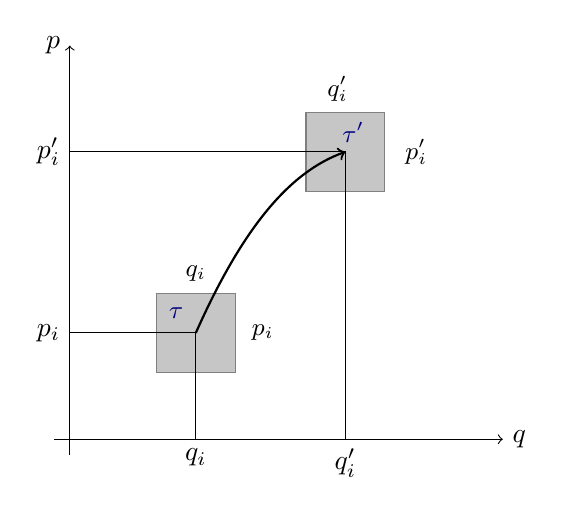
\begin{tikzpicture}[x=1cm,y=1cm]
  \draw[->] (0,-0.2) -- (0,5) node[left] {$p$};
  \draw[->] (-0.2,0) -- (5.5,0) node[right] {$q$};
  % dolní element
  \fill[gray!45] (1.1,0.85) rectangle (2.1,1.85);
  \draw[gray] (1.1,0.85) rectangle (2.1,1.85);
  \node[NavyBlue] at (1.35,1.6) {\small $\dd\tau$};
  \node at (1.6,2.1) {\small $\dd q_i$};
  \node at (2.45,1.35) {\small $\dd p_i$};
  % horní element
  \fill[gray!45] (3,3.15) rectangle (4,4.15);
  \draw[gray] (3,3.15) rectangle (4,4.15);
  \node[NavyBlue] at (3.6,3.9) {\small $\dd\tau'$};
  \node at (3.4,4.45) {\small $\dd q_i'$};
  \node at (4.4,3.65) {\small $\dd p_i'$};
  % souřadnice
  \draw (0,1.35) -- (1.6,1.35) -- (1.6,0);
  \draw (0,3.65) -- (3.5,3.65) -- (3.5,0);
  \node[left] at (0,1.35) {$p_i$};
  \node[left] at (0,3.65) {$p_i'$};
  \node[below] at (1.6,0) {$q_i$};
  \node[below] at (3.5,0) {$q_i'$};
  % trajektorie
  \draw[->,thick] (1.6,1.35) .. controls (2.2,2.7) and (2.8,3.4) .. (3.5,3.65);
\end{tikzpicture}
\end{minipage}
\begin{minipage}{0.53\textwidth}
\underline{$t\to t' = t + \dd t$}
\begin{align*}
  q_i' &= q_i + \dot q_i\,\dd t + \mathcal O(\dd t^2) \\
  p_i' &= p_i + \dot p_i\,\dd t + \mathcal O(\dd t^2)
\end{align*}
\begin{align*}
  \textcolor{NavyBlue}{\textcircled{$*$}}\quad
  \dd q_i' &= \dd q_i + \pdv{\dot q_i}{q_i}\dd q_i\,\dd t + \mathcal O(t^2) \\
  \dd p_i' &= \dd p_i + \pdv{\dot p_i}{p_i}\dd p_i\,\dd t + \mathcal O(t^2)
\end{align*}
\end{minipage}

\textcolor{OliveGreen}{\textit{d/dp(dq/dt)=0 \dots\ prohoď derivace\dots}}
\hfill
\textcolor{NavyBlue}{\small \textcircled{$*$} \ $q_i\pm\tfrac12\dd q_i \xrightarrow{\,t+\dd t\,} q_i\pm\tfrac12\dd q_i + \big(\dot q_i \pm \tfrac12\pdv{\dot q_i}{q_i}\dd q_i\big)\dd t$}

\begin{itemize}
  \item systémy původně v $\dd\tau$ se přesunou do $\dd\tau'$:
  \[
    \prod_i\dd p_i\,\dd q_i \to \prod_i\dd p_i'\,\dd q_i' = \prod_i\dd p_i\,\dd q_i\Big[1 + \Big(\pdv{\dot q_i}{q_i} + \pdv{\dot p_i}{p_i}\Big)\dd t + \mathcal O(t^2)\Big]
  \]
  \item vývoj mikrostavu se řídí Ham.\ rovnicemi
  \[
    \Rightarrow\quad \pdv{\dot q_i}{q_i} = \pdv{q_i}\Big(\pdv{H}{p_i}\Big);\quad
    \pdv{\dot p_i}{p_i} = \pdv{p_i}\Big(-\pdv{H}{q_i}\Big)
    \quad\&\quad \frac{\partial^2H}{\partial p_i\partial q_i} = \frac{\partial^2H}{\partial q_i\partial p_i}
  \]
  \[
    \Rightarrow\quad \vzorec{\dd\tau = \dd\tau'}
  \]
  $\Rightarrow$ \kw{OBJEM FÁZOVÉHO PROSTORU JE DYNAMICKÝ INVARIANT}
  \item přitom počet stavů $\dd\mathcal N$ v daném fázovém objemu se nemohl změnit
  \[ \Rightarrow\quad w(p',q',t')\,\dd\tau' = w(p,q,t)\,\dd\tau \]
\end{itemize}

%----------------------------------------------------------------------
\strana{L09-4}
{\color{NavyBlue}
\textbf{Podrobněji (doplněk):}
\[
  q + \tfrac12\delta q \xrightarrow{\ t\to t+\dd q\ } q + \tfrac12\delta q + \frac{\dd}{\dd t}\big(q + \tfrac12\delta q\big)\dd t =
\]
\[
  \Big/\ \delta q = \pdv{q}{q}\dd q + \underset{\nwarrow\,0!}{\pdv{q}{p}}\dd p = \dd q\ \Big/
\]
\begin{align*}
  &= \big(q + \tfrac12\delta q\big) + \dot q\,\dd t + \tfrac12\Big[\pdv{\dot q}{q}\dd q + \pdv{\dot q}{p}\dd p\Big]\dd t \\
  &= \big(q + \tfrac12\dd q\big) + \dot q\,\dd t + \tfrac12\pdv{\dot q}{q}\dd q\,\dd t
\end{align*}
\[
  q \to q + \dot q\,\dd q \quad\Rightarrow\quad \delta q = \dd q \to \dd q + \pdv{\dot q}{q}\dd q\,\dd t = \Big(1 + \pdv{\dot q}{q}\dd t\Big)\dd q \ \underset{+\mathcal O(t^2)}{}
\]
\[
  \Rightarrow\quad \dd q\,\dd p \to \Big(1 + \Big[\pdv{\dot q}{q} + \pdv{\dot p}{p}\Big]\dd t\Big)\dd q\,\dd p = \dd p\,\dd q \quad\checkmark
\]
\[
  \dot q = \pdv{H}{p} \quad\&\quad \dot p = -\pdv{H}{p} \quad\Rightarrow\quad
  [\ ] = \frac{\partial^2H}{\partial q\partial p} - \frac{\partial^2H}{\partial p\partial q} = 0
\]
}

\medskip
{\color{OliveGreen}
\underline{Skutečný důkaz:}
\begin{itemize}
  \item[$\to$] geom.\ formulace anal.\ mechaniky
  \item[$\to$] čas.\ vývoj jako spec.\ případ kanonické transformace $\Rightarrow$ $\mathrm{Jac} = 1$ \quad [Landau, Lifšic; Brdička, Hladík]
\end{itemize}
}

%----------------------------------------------------------------------
\strana{L09-5}
\providecommand{\skrt}[1]{\tikz[baseline=(X.base)]{\node[inner sep=0pt](X){$\displaystyle #1$};\draw[NavyBlue](X.south west)--(X.north east);}}

\begin{veta}[Liouvilleův teorém]
Hustota stavů $w(p,q,t)$ ve fázovém prostoru se chová jako \kw{nestlačitelná kapalina}.

\smallskip
{\color{OliveGreen}\small\itshape Systém částic, jejichž okamžitý stav je reprezentován body ve fázovém prostoru, se chová jako deformovatelné těleso, jehož objem ovšem zůstává beze změny. (Jacobiho determinant kanonické transformace je 1 a vývoj mech.\ systému lze interpretovat jako speciální kanonickou transformaci (i)$\to$(f) (Podolský/Brdička, Hladík)) \hfill DK Landau, Lifsic nebo geom.\ metody}
\end{veta}

\begin{minipage}{0.2\textwidth}
\[ \vzorec{\frac{\dd w}{\dd t} = 0} \]
\end{minipage}
\begin{minipage}{0.78\textwidth}
\hfill Joseph Liouville, 1809--1882 (Fra, mat.) \\
{\color{OliveGreen}\small\itshape zde tato rovnice znamená, že se posadíme na jeden konkrétní systém z našeho souboru a sledujeme, jak se kolem nás mění hustota psti/hustota systémů\dots\ ve $w(p,q,t)$ v principu $p,q$ na čase nezávisí, ale vždy to můžeme takto interpretovat\dots}
\end{minipage}

\begin{itemize}
  \item explicitně: \quad $\big(p = p(t)\ \Rightarrow\ p' = p(t+\dd t), \dots\big)$
  \[
    w\big(p(t+\dd t), q(t+\dd t), t+\dd t\big) = w(p,q,t)
  \]
  \[
    \Rightarrow\quad \vzorec{\frac{\dd w}{\dd t} = \pdv{w}{t} + \sum_{i=1}^{3N}\Big(\pdv{w}{q_i}\dot q_i + \pdv{w}{p_i}\dot p_i\Big)\dd t = 0} \qquad (*)
  \]
  \item Hamiltonovy rovnice
  \[
    \vzorec{\pdv{w}{t} = \pdv{H}{q_i}\pdv{w}{p_i} - \pdv{H}{p_i}\pdv{w}{q_i} = \{H,w\}}
    \quad\leftarrow\ \text{\kw{Poissonova závorka}}
  \]
\end{itemize}

\begin{minipage}{0.55\textwidth}
\begin{itemize}
  \item rovnice $(*)$ je \underline{rovnice kontinuity}
  \[ \pdv{w}{t} + \nabla(w\,v) = 0 \]
  \begin{itemize}
    \item[$\to$] $v = \{\dot q_i,\dot p_i \mid i = 1,\dots,3N\}$
    \item[$\to$] $\nabla = \big\{\pdv{q_i},\pdv{p_i} \mid i = 1,\dots,3N\big\}$
    \item[$\to$] příspěvek $w\nabla v$ vymizí ($\Leftarrow$ Ham.\ rovnice)
  \end{itemize}
\end{itemize}
\end{minipage}
\hfill
\begin{minipage}{0.42\textwidth}
\begin{tcolorbox}[colback=white,colframe=NavyBlue,boxrule=0.6pt,arc=0pt,left=3pt,right=3pt]
\color{NavyBlue}\small
Liouvilleův teorém je důvod, proč je fázový prostor (a ne např.\ rychlostní fázový prostor) ten správný prostor pro mikroskopický popis makrosystému a proč je objem dostupné části fázového prostoru správnou mírou entropie (viz dále).
\end{tcolorbox}
\end{minipage}

\begin{itemize}
  \item časový \underline{vývoj střední hodnoty} $F(p,q)$:
  \[
    \frac{\dd}{\dd t}\langle F\rangle = \frac{\dd}{\dd t}\int\dd\tau_N\,w(p,q,t)\,F(p,q) = \int\dd\tau_N\,\pdv{w(p,q,t)}{t}F(p,q)
  \]
  \hfill
  \begin{minipage}{0.45\textwidth}
  {\color{OliveGreen}\small\itshape neboli zde už opět $p,q$ na čase nezávisí} \\
  {\color{NavyBlue}\small pod integrálem je opravdu $\pdv{w}{t}$, nikoliv $\frac{\dd w}{\dd t}$ \dots\ integrujeme přes celý prostor, zajímá nás, jak se $w$ mění v každém bodě}
  \end{minipage}
  \[
    \Rightarrow\quad \frac{\dd}{\dd t}\langle F\rangle = \int\dd\tau_N\,\{H,w\}\,F(p,q)
  \]
  \begin{itemize}
    \item per partes:
  \end{itemize}
  \begin{align*}
    \int\dd\tau_N\Big(\pdv{H}{q}\pdv{w}{p} - \pdv{H}{p}\pdv{w}{q}\Big)F(p,q)
    &= \Big[\pdv{H}{q}\,w\,F(p,q)\Big]_{p=-\infty}^{\infty} - \Big[\pdv{H}{p}\,w\,F\Big]_{q=-\infty}^{\infty} \\
    &\quad - \int\dd\tau_N\,w\Big[\skrt{\frac{\partial^2H}{\partial p\partial q}F} + \pdv{H}{q}\pdv{F}{p}
       - \skrt{\frac{\partial^2H}{\partial q\partial p}F} - \pdv{H}{p}\pdv{F}{q}\Big]
  \end{align*}
\end{itemize}

%----------------------------------------------------------------------
\strana{L09-6}
\[
  \Rightarrow\quad \vzorec{\frac{\dd}{\dd t}\langle F\rangle = -\int\dd\tau_N\,w\,\{H,F\} = \big\langle\{F,H\}\big\rangle}
  = \int\dd\tau_N\,\{H,w\}\,F(p,q)
\]
\begin{itemize}
  \item střední hodnoty integrálů pohybu ($\equiv\{F,H\} = 0$) se pro lib.\ $w$ nemění $\Rightarrow$ konzistentní výsledek
  \item \underline{ale:} v \underline{rovnovážném stavu} se nemění střední hodnoty \underline{žádných} makroskopicky pozorovatelných veličin
\end{itemize}

\begin{minipage}{0.52\textwidth}
{\color{OliveGreen}\small\itshape OK, je-li $F$ integrál pohybu, potom $\langle F\rangle$=konst bez ohledu na $w$; Ano, např.\ energie systému se zachovává i mimo rovnováhu, tedy pro $\dd w/\dd t\neq 0$. My chceme, aby se zachovávaly střední hodnoty všech pozorovatelných, tedy $\{w,H\} = 0$.

\smallskip
Co potom můj opakovaný argument, že relevantní TD veličiny jsou ty spojené s integrály pohybu? Myslím, že je to OK -- mohu počítat střední hodnoty libovolné veličiny, ale $w$ závisí jen na integrálech pohybu $\to$ makrostav je plně určen jejich hodnotami.}
\end{minipage}
\hfill
\begin{minipage}{0.45\textwidth}
\begin{veta}[Rovnováha]
\[
  \pdv{w_{\mathrm{eq}}}{t} = 0 \ \Leftrightarrow\ \vzorec{\{w_{\mathrm{eq}},H\} = 0}
\]
pro rovnovážnou hustotu pravděpodobnosti
\end{veta}
\end{minipage}

\pozor{!} Především jsme ukázali, že platí
\[
  \{w_{\mathrm{eq}},H\} = 0 \quad\Rightarrow\quad \big\langle\underbrace{\{F,H\}}_{=\,\dot F}\big\rangle = 0 \quad\text{i pro } \{F,H\}\neq 0
\]

\begin{veta}[Důsledek]
Rovnovážná hustota pravděpodobnosti může záviset pouze na \kw{integrálech pohybu} $C_n$: \quad $\{C_n,H\} = 0$!
\begin{align*}
  w(p,q) = w\big(C_n(p,q)\big) \ \Rightarrow\ \{w,H\} &= \pdv{w}{q}\pdv{H}{p} - \pdv{w}{p}\pdv{H}{q} \\
  &= \pdv{w}{C_n}\Big(\pdv{C_n}{q}\pdv{H}{p} - \pdv{C_n}{p}\pdv{H}{q}\Big) = 0 \quad\checkmark
\end{align*}
\end{veta}
\begin{itemize}
  \item takovým integrálem pohybu je vždy energie: \quad $\{H,H\} = 0$ \qquad \textcolor{Red}{!\,izolovaný systém!}
  \item existence dalších integrálů pohybu závisí na symetrii systému.
  \begin{itemize}
    \item[--] celk.\ hybnost \& moment hybnosti obvykle nejsou relevantní, příslušné makroskopické toky můžeme odtransformovat
  \end{itemize}
\end{itemize}

%----------------------------------------------------------------------
\strana{L09-7}
\begin{itemize}
  \item tento důsledek nás přivádí k \underline{axiomu stejných pravděpodobností}:
  \begin{itemize}
    \item[$\to$] v izolovaném systému je celková energie konst.
    \item[$\Rightarrow$] $\forall$ mikrostavy splňují $H(p,q) = E$
    \item[$\Rightarrow$] pokud $w = w(E)$, musí být $\forall$ mikrostavy stejně pravděpodobné (pro \underline{$V,N$} fixní) \\
          \hfill \textcolor{NavyBlue}{$V,N$ definují samotný fáz.\ prostor!}
  \end{itemize}
\end{itemize}

\underline{Obecněji:}
\begin{veta}[Princip stejných pravděpodobností]
Pokud nemáme žádnou další informaci, považujeme všechny mikrostavy kompatibilní s daným makrostavem za stejně pravděpodobné.

\textcolor{Red}{$\to$ výchozí axiom SF, musí být ověřen experimentem}
\end{veta}

\begin{itemize}
  \item mohu tedy psát
  \[
    w(p,q;E,V,N) = \begin{cases} \dfrac{1}{W} & H(p,q) = E \\[4pt] 0 & \text{jinak} \end{cases}
    \qquad ?
    \qquad\qquad
    \begin{array}{c}
      \textcolor{NavyBlue}{W\ \dots\ \text{norma:}} \\
      \textcolor{NavyBlue}{\int w\,\dd\tau_N = 1} \\
      \textcolor{Red}{\downarrow}
    \end{array}
  \]
  \textcolor{OliveGreen}{$\displaystyle w(p,q;E,V,N) = \frac1W\,\delta\big(E - H(p,q)\big)$}
  \hfill
  $\textcolor{Red}{\displaystyle W = \Sigma(E,V,N) = \int\dd\tau_N\,\delta\big[E - H(p,q)\big]}$
  \item jak vypadá odpovídající funkcionál entropie?
  \[
    \vzorec{S = k\log W} \quad\dots\ \text{\kw{Boltzmannova entropie}}
  \]
  \hfill (jak ji ovšem zapsal Planck) \hfill\null

  $W$ -- Wahrscheinlichkeit (\uv{pravděpodobnost})
  \begin{itemize}
    \item[--] míra pravděpodobnosti makrostavu \dots\ také permutabilita \\
          ($\sim$ počet mikrostavů, které daný $M$ mohou realizovat)
  \end{itemize}
  \item motivováno představou ireverzibility jako přechodu k pravděpodobnějšímu makrostavu
  \item proč $\log$:
  \begin{enumerate}[label=\arabic*)]
    \item monotónní $\Rightarrow$ $\max W \Leftrightarrow \max S$
    \item aditivita entropie: neinteragující podsystémy
    \[ \Rightarrow\quad W = W_1\cdot W_2 \quad\Rightarrow\quad S = S_1 + S_2 \]
  \end{enumerate}
\end{itemize}

%----------------------------------------------------------------------
\strana{L09-8}
\subsection{Entropie id.\ plynu}
\begin{minipage}{0.45\textwidth}
\begin{itemize}
  \item studujme složený systém
  \begin{align*}
    E_1 + E_2 &= E \\
    N_1 + N_2 &= N \\
    V_1 + V_2 &= V
  \end{align*}
\end{itemize}
\end{minipage}
\begin{minipage}{0.53\textwidth}
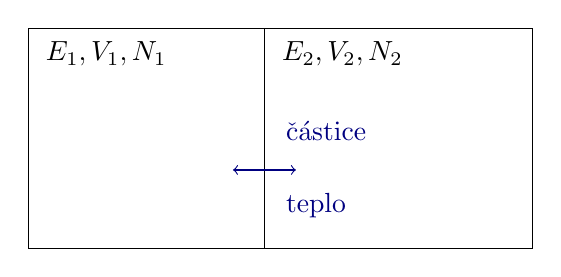
\begin{tikzpicture}[x=1cm,y=1cm]
  \draw (0,0) rectangle (6.4,2.8);
  \draw (3,0) -- (3,2.8);
  \node[anchor=north west] at (0.1,2.75) {$E_1, V_1, N_1$};
  \node[anchor=north west] at (3.1,2.75) {$E_2, V_2, N_2$};
  \draw[NavyBlue,<->] (2.6,1.0) -- (3.4,1.0);
  \node[NavyBlue,anchor=west] at (3.15,1.5) {částice};
  \node[NavyBlue,anchor=west] at (3.15,0.55) {teplo};
\end{tikzpicture}
\end{minipage}

\begin{itemize}
  \item \underline{mikroskopický model}
  \[
    H(\{p_i,q_i\}) = \sum_{i=1}^{3N}\frac{p_i^2}{2m} \qquad p_i\in(-\infty,\infty) \qquad q_i\in V
  \]
  \item termodynamický popis: \quad $E, V, N, E_1, V_1, N_1$
\end{itemize}

\underline{Předpoklady:}
\begin{enumerate}[label=\arabic*)]
  \item \underline{nezávislost $p_i$ a $q_i$} \dots\ hybnost částice nezávisí (není korelována s) její poloze
  \[ \Rightarrow\quad w(p_i,q_i) = w_p(\{p_i\})\,w_q(\{q_i\}) \]
  \underline{NB:} $p_i$ nezávislé nejsou, svazuje je $\sum\frac{p_i^2}{2m} = E$
  \item \underline{rozlišitelnost částic} \dots\ mají stejné vlastnosti, ale v principu je možné sledovat individuální trajektorie
  \begin{itemize}
    \item[--] nerozlišitelnost je \uv{kvantová} vlastnost, na klasické úrovni nedává dobrý smysl
  \end{itemize}
\end{enumerate}
\begin{itemize}
  \item předpoklad 1 činí z poloh a hybností nezávislé podsystémy
  \[
    \Rightarrow\ \text{očekávám}\quad
    S(E,V,N) = \underset{\substack{\nearrow\\ \textcolor{NavyBlue}{\text{hybnostní}}}}{S_p(E,N)} + \underset{\substack{\nwarrow\\ \textcolor{NavyBlue}{\text{konfigurační}}}}{S_q(V,N)}
    \qquad \textcolor{NavyBlue}{\text{entropie}}
  \]
\end{itemize}

%----------------------------------------------------------------------
\strana{L09-9}
{\color{NavyBlue}
\[
  H = \sum_{i=1}^{3N}\frac{p_i^2}{2m} \quad\&\quad
  \underset{V = L^3}{q_i\in(-L/2,L/2)},\ p_i\in(-\infty,+\infty) \ \Leftarrow\ H,\ T^*Q
\]
\begin{align*}
  \Sigma(E,V,N) &= \int\dd^{3N}p_i\,\dd^{3N}q_i\,\delta\Big(E - \sum\frac{p_i^2}{2m}\Big) \\
  &= V^N\int\dd^{3N}p_i\,\delta\Big(E - \sum\frac{p_i^2}{2m}\Big)
     = \Big/\ \frac{p_i}{(2m)^{1/2}} = x_i \quad \dd p_i = (2m)^{1/2}\dd x_i\ \Big/ \\
  &= V^N(2m)^{\frac{3N}{2}}\int\dd^{3N}x_i\,\delta\Big(E - \sum x_i^2\Big)
     = \Big/\ \sum x_i^2 = x^2 \ \text{(hypersfér.\ souř.)}\ \Big/ \\
  &= V^N(2m)^{\frac{3N}{2}}\int_0^\infty x^{3N-1}\delta(E - x^2)\,\dd x\
     \underbrace{\int\mathrm{Jac}(\vec\vartheta)\,\dd^{3N-1}\vartheta}_{\substack{\text{povrch jednotkové}\\ \text{3N-dim.\ sféry}\\ S_{3N}(1)}} \\
  &= \big/\ x^2 = y \quad 2x\,\dd x = \dd y\ \big/ \\
  &= V^N(2m)^{\frac{3N}{2}}S_{3N}(1)\cdot\frac12\int_0^\infty y^{\frac{3N}{2}-1}\delta(E - y)\,\dd y
\end{align*}
\[
  \Sigma = V^N(2m)^{\frac{3N}{2}}S_{3N}(1)\cdot\frac12(E)^{\frac{3N}{2}-1}
\]
\[
  \Rightarrow\quad \vzorec{\Sigma(E,V,N) = m\,V^NS_{3N}(1)\,(2mE)^{\frac{3N}{2}-1}}
\]
}

\textcolor{OliveGreen}{$S_{3N}(1)$:} \quad
{\color{BurntOrange}
$\displaystyle\int_{\mathbb R^{3N}}\dd^{3N}x_i\,e^{-\sum x_i^2} = \Big(\int_{-\infty}^{\infty}\dd x_i\,e^{-x_i^2}\Big)^{3N} =
\underset{\substack{\textcolor{Red}{\uparrow\ \text{počítej}}\\ \textcolor{Red}{(\int_{-\infty}^{\infty})^2}}}{\pi^{\frac{3N}{2}}}$
\[
  \rotatebox{90}{$=$}
\]
\[
  \underbrace{\int_0^\infty x^{3N-1}e^{-x^2}\dd x}_{=\,\frac12\Gamma(\frac{3N}{2})}\
  \underbrace{\int\mathrm{Jac}(\vec\vartheta)\,\dd^{3N-1}\vartheta}_{S_{3N}(1)}
  = \frac12\Gamma\Big(\frac{3N}{2}\Big)S_{3N}(1)
\]
\textcolor{Red}{$\Big/\ \Gamma(z) = \displaystyle\int_0^\infty t^{z-1}e^{-t}\ \Big/$} \ $x^2 = t$, $2x\,\dd x = \dd t$
\[
  \frac12\int 2x\,\dd x\,x^{3N-2}e^{-x^2} = \frac12\int\dd t\,t^{\frac{3N}{2}-1}e^{-t} = \frac12\Gamma\Big(\frac{3N}{2}\Big)
\]
}
\[
  \textcolor{OliveGreen}{\Downarrow}\qquad
  \vzorec{S_{3N}(1) = \frac{2\pi^{\frac{3N}{2}}}{\Gamma\big(\frac{3N}{2}\big)}}
\]

%----------------------------------------------------------------------
\strana{L09-10}
{\color{NavyBlue}
\[
  \Rightarrow\quad \Sigma(E,V,N) = m\,V^N\frac{2\pi^{\frac{3N}{2}}}{\Gamma\big(\frac{3N}{2}\big)}(2mE)^{\frac{3N}{2}-1}
\]
\[
  \Gamma\Big(\frac{3N}{2}\Big) = \Big(\frac{3N}{2} - 1\Big)! \quad\&\quad \text{Stirling: } \log n! = n\log n - n
\]

přesněji: metoda sedl.\ bodu
\[
  n! = \Gamma(n+1) = \int\dd t\,t^ne^{-t} = \int\dd t\,e^{-t+n\log t} = \int\dd t\,e^{g(t)}
\]
\[
  g(t) = n\log t - t = \Big/\ \textcolor{BurntOrange}{\text{Taylor kolem max:}}
\]
{\color{BurntOrange}
\[
  0 = g'(t_0) = \frac{n}{t_0} - 1 \ \Rightarrow\ n = t_0 \ \Rightarrow\ g(t) = n\log n - n + \tfrac12g''(n)(t-n)^2
\]
\[
  g'' = -\frac{n}{t^2}\Big|_{t=n} = -\frac1n \ \Rightarrow\ g(t) \sim n\log n - n - \frac{(t-n)^2}{2n}
\]
}
\[
  \Rightarrow\quad n! \simeq \frac12e^{n\log n - n}\int_{-\infty}^{\infty}e^{-\frac{(t-n)^2}{2n}}\dd t = \frac12n^ne^{-n}(2\pi n)^{1/2}
\]
\[
  \Rightarrow\quad n! = \Big(\frac{\pi n}{2}\Big)^{1/2}n^ne^{-n} \ \Rightarrow\
  \log n! = n\log n - n + \underbrace{\tfrac12\log n + \tfrac12\log\tfrac{\pi}{2}}_{\text{irelevantní}}
\]
\begin{align*}
  \log\Gamma\Big(\frac{3N}{2}\Big) &= \Big(\frac{3N}{2} - 1\Big)\log\Big(\frac{3N}{2} - 1\Big) - \frac{3N}{2} + 1
  = \frac{3N}{2}\Big(1 - \frac{2}{3N}\Big)\log\Big[\frac{3N}{2}\Big(1 - \frac{2}{3N}\Big)\Big] \\
  &\quad - \frac{3N}{2} + 1 \overset{N\to\infty}{\sim} \frac{3N}{2}\log\frac{3N}{2} - \frac{3N}{2}
\end{align*}
\[
  \Sigma(E,V,N) = m\,V^N\frac{2\pi^{\frac{3N}{2}}}{\Gamma\big(\frac{3N}{2}\big)}(2mE)^{\frac{3N}{2}-1} =
\]
\begin{align*}
  \Rightarrow\ S(E,V,N) = k_B\log\Sigma &= N\log V + \frac{3N}{2}\log\pi + \frac{3N}{2}\Big(1 - \textcolor{Red}{\sout{\tfrac{2}{3N}}}\Big)\log(2mE) \\
  &\quad - \frac{3N}{2}\log\frac{3N}{2} + \frac{3N}{2} \\
  &= \underbrace{N\log\big[VE^{3/2}N^{-3/2}\big]}_{\substack{\Downarrow\\ \text{\pozor{není extenzivní!}}}}
   + \underbrace{N\log\Big[\pi^{3/2}(2m)^{3/2}\Big(\frac32\Big)^{-3/2}\Big] + \frac32N}_{Ns_0}
\end{align*}
}

\textcolor{NavyBlue}{\textbf{oprava:}} \quad
$\textcolor{Red}{\dd\tau_N = \dd^{3N}p\,\dd^{3N}q}$ \ $\to$ \
$\displaystyle\dd\tau_N = \textcolor{OliveGreen}{\frac{1}{N!}}\prod_{i=1}^{3N}\frac{\dd p\,\dd q}{\textcolor{BurntOrange}{h}}$
\quad
\begin{minipage}{5.2cm}\small
\textcolor{OliveGreen}{$\nearrow\ \frac{1}{N!}$ \dots\ nerozliš.\ částic} \\
\textcolor{BurntOrange}{$\searrow\ \frac1h$ \dots\ počítání kvant.\ stavů (cf.\ rel.\ neurčitosti)}
\end{minipage}

%----------------------------------------------------------------------
\strana{L09-11}
\subsubsection*{A) Konfigurační entropie \quad \textcolor{Red}{\Large OBSOLETE!}}
\begin{itemize}
  \item $w_1(q_i) = \text{konst}$ \dots\ pst.\ nalezení lib.\ částice kdekoliv v boxu je stejná
  \begin{itemize}
    \item[$\Rightarrow$] pst.\ jejího nalezení ve $V_1$ je $V_1/V$ a ve $V_2$ je $V_2/V = 1 - \frac{V_1}{V}$
  \end{itemize}
  \item[$\Rightarrow$] pravděpodobnost makrostavu $M(V_1,N_1,V_2 = V - V_1,N_2 = N - N_1)$ je dána binomickým rozdělením
\end{itemize}

\begin{minipage}{0.62\textwidth}
\[
  W_q(N_1|N) = \frac{N!}{N_1!\,N_2!}\Big(\frac{V_1}{V}\Big)^{N_1}\Big(\frac{V_2}{V}\Big)^{N_2}
\]
\end{minipage}
\begin{minipage}{0.36\textwidth}
\begin{tcolorbox}[colback=white,colframe=NavyBlue,boxrule=0.6pt,arc=0pt,left=2pt,right=2pt]
\color{NavyBlue}
\begin{align*}
  w &= \tbinom{N}{n}p^nq^{N-n} \\
  \langle n\rangle &= Np \\
  \sigma^2 &= \langle n^2\rangle - \langle n\rangle^2 = Npq
\end{align*}
\end{tcolorbox}
\end{minipage}

\textcolor{NavyBlue}{\underline{NB:} $\displaystyle\sum_{N_1=0}^{N}W_q(N_1|N) = \binom{N}{N_1}\Big(\frac{V_1}{V}\Big)^{N_1}\Big(1 - \frac{V_1}{V}\Big)^{N-N_1} = \Big(\frac{V_1}{V} + 1 - \frac{V_1}{V}\Big)^N = 1$}

\begin{itemize}
  \item střední hodnota: \quad $\langle N_1\rangle = N\dfrac{V_1}{V}$ \ $\Leftrightarrow$ \ $\langle N_2\rangle = N\dfrac{V_2}{V}$ \ $\Rightarrow$ \ $\dfrac{\langle N_1\rangle}{V_1} = \dfrac{\langle N_2\rangle}{V_2} = \dfrac{N}{V}$
  \item \underline{rozptyl:} \quad $(\Delta N_1)^2 = N\dfrac{V_1}{V}\Big(1 - \dfrac{V_1}{V}\Big) = \langle N_1\rangle\dfrac{V_2}{V}$
  \[
    \Rightarrow\quad \vzorec{\frac{\Delta N_1}{\langle N_1\rangle} \propto \langle N_1\rangle^{-1} \propto N^{-1/2}} \qquad \text{\pozor{!}}
  \]
\end{itemize}
\begin{enumerate}[label=\arabic*)]
  \item fluktuace počtu částic jsou pro $N\sim 10^{26}$ zanedbatelné vůči celk.\ počtu částic:
  \[ \langle N_1\rangle\sim 10^{26} \ \Rightarrow\ \Delta N_1\sim 10^{13} \ \dots\ \text{v zásadě neměřitelné} \]
  \item $W_q(N_1|N)$ můžeme aproximovat normálním rozdělením -- viz centrální limitní věta \\
        $\Downarrow$ rozdělení je symetrické okolo $\langle N_1\rangle$
  \item[\pozor{!}\,3)] $\langle N_1\rangle \cong$ modus $N_1$ \quad [$\Leftrightarrow\max W(N_1|N)$]
\end{enumerate}
$\Rightarrow$ funguje termodynamický princip maxima: striktně vzato pozorujeme střední hodnotu, ale tu lze ztotožnit s modem pstního rozdělení $\Rightarrow$ \underline{realizuje se nejpravděpodobnější stav}

$\Rightarrow$ má tedy opravdu smysl ztotožnit entropii s nějakou monot.\ fcí $W_q(N_1|N)$

\begin{itemize}
  \item \underline{def:}
  \begin{enumerate}[label=\arabic*)]
    \item $\Sigma_q(N,V) \equiv \dfrac{V^N}{N!}$ \quad $\Rightarrow$ \quad $W_q(N_1|N) = \dfrac{\Sigma_q(N_1,V_1)\,\Sigma_q(N_2,V_2)}{\Sigma_q(N,V)}$
    \item $S_q(N,V) = k\log\dfrac{\Sigma_q(N,V)}{\underset{\textcolor{NavyBlue}{\nwarrow\ \text{lib.\ konst.\ pro bezrozměrnost argumentu log}}}{b}} + Ns_q$
  \end{enumerate}
\end{itemize}

%----------------------------------------------------------------------
\strana{L09-12}
\hfill \textcolor{Red}{\large OBSOLETE}
\[
  \log W_q(N_1|N) = S_q(N_1,V_1) + S_q(N_2,V_2) - \underbrace{S_q(N,V)}_{\textcolor{NavyBlue}{\text{pro izol.\ systém konstanta!}}}
\]
$\Rightarrow$ definuji entropii slož.\ systému
\[
  \vzorec{S_q^{(1,2)}(N_1,V_1,N_2,V_2) = S_q(N_1,V_1) + S_q(N_2,V_2) = S_q(N,V) + \log W_q(N_1|N)}
\]
\textcolor{NavyBlue}{\small $\uparrow$ je silný předpoklad, že $S^{(1,2)} = S^{(1)} + S^{(2)}$, jakkoliv je pro neinterag.\ systémy na základě TD přirozený (je dobré si stále uvědomovat, že míříme ke známému cíli, abychom \uv{odvození} nepřeceňovali)}

\begin{itemize}
  \item z konstrukce vyplývá, že maximalizací $S_q^{(1,2)}$ s vazbou $N_2 = N - N_1$ dostaneme $N_1^{\mathrm{eq}} = \langle N_1\rangle = \frac{N}{V}V_1 = N_1^{\mathrm{mod}}$ \quad [$S_q(N,V)$ na RHS je konstanta]
  \item pro makroskop.\ $N$ je $W_q(N_1|N)$ normální rozdělení
  \[
    W_q(N_1|N) = \frac{1}{\sqrt{2\pi\sigma^2}}\exp\Big(-\frac{(N_1 - \langle N_1\rangle)^2}{2\sigma^2}\Big) \qquad\text{kde } \sigma^2\propto\langle N_1\rangle\propto N
  \]
  \[
    \Rightarrow\quad \log W_q \sim -\frac12\log N - \frac{(N_1 - \langle N_1\rangle)^2}{N}
  \]
  \item v rovnováze $N_1\sim\langle N_1\rangle$ \quad $\Rightarrow$ \quad $\vzorec{\log W_q \sim -\frac12\log N \ll S_q(N,V)}$
\end{itemize}

{\color{NavyBlue}
\underline{Stirling:} $N!\sim N\log N - 1$ \ $\Rightarrow$ \ $S_q(N,V) = kN\log\frac{V}{Nb} + N(s_q + 1)$

\underline{NB:} Stirlingova formule
\begin{enumerate}[label=\alph*)]
  \item $N! = \Gamma(N+1) = \int_0^\infty e^{-x}x^N\dd x$ \ \& \ metoda sedlového bodu \\
        $\Rightarrow$ $N! \simeq \sqrt{2\pi N}\,N^Ne^{-N}$ \quad (+ lze odvodit další korekce)
  \item $\log N! = \log\Big(\prod_{n=1}^{N}n\Big) = \sum_{n=1}^{N}\log n \approx \int_1^N\dd x\log x = N\log N - N + \underset{\ll N}{1}$ \\
        $\Rightarrow$ $N! \simeq N^Ne^{1-N}$
\end{enumerate}
\begin{itemize}
  \item Gosper: \quad $N! \simeq N^Ne^{-N}\sqrt{\big(2N + \frac13\big)\pi}$
\end{itemize}
}

\begin{itemize}
  \item v rovnováze tedy platí
  \[
    S_q^{(1,2)}(V_1,N_1,V_2,N_2) = S_q(V_1,N_1) + S_q(V_2,N_2) = S_q(V,N) + \mathcal O(\log N)
  \]
\end{itemize}
\pozor{!} očekávaný výsledek: přepážka propouští částice $\Rightarrow$ rovn.\ stav je stejný, jako kdyby tam vůbec nebyla (rozdělení na podsystémy může být jen myšlené)
\begin{itemize}
  \item celkem pro $N\gg 1$: \quad
  $\vzorec{S_q(N,V) = kN\log\Big(\frac{V}{V_0}\frac{N_0}{N}\Big) + Ns_q}$
\end{itemize}

%----------------------------------------------------------------------
\strana{L09-13}
\subsubsection*{B) Příspěvek od hybností \quad \textcolor{Red}{\large OBSOLETE}}
\begin{itemize}
  \item pro odvození $S_p(E,N)$ předpokládejme diatermální stěnu, která nepropouští částice $\Rightarrow$ $N_1, N_2$ jsou fixní (jinak bychom znovu řešili i výměnu částic)
  \[
    \Rightarrow\quad E_1 = \sum_{i=1}^{N_1}\frac{p_i^2}{2m} \quad\&\quad E_2 = \sum_{j=N_1+1}^{N}\frac{p_j^2}{2m} = \sum_{j=1}^{N_2}\frac{p_j^2}{2m} \quad\&\quad E = E_1 + E_2
  \]
  \item princip stejných pravděpodobností: libovolný mikrostav realizující stejné rozdělení energie $E = E_1 + E_2$ je stejně pravděpodobný
  \begin{itemize}
    \item[$\Rightarrow$] libovolné rozdělení energie $E_1$ mezi $3N_1$ hybností je stejně pravděpodobné a totéž ve 2.\ podsystému
  \end{itemize}
  \[
    \Rightarrow\quad W_p(E_1|E) = \frac{\Sigma_p(E_1,N_1)\,\Sigma_p(E_2,N_1)}{\Sigma_p(E,N)}
  \]
  \begin{itemize}
    \item[$\to$] míra pravděpodobnosti makrostavu je úměrná objemu dostupného fáz.\ prostoru vymezeného danou energií
    \item[$\to$] $\Sigma_p(E,N)$ je \uv{normalizační konstanta}
  \end{itemize}
  \[
    \Sigma_p(E,N) = \int_{\sum_i\frac{p_i^2}{2m} = E}\prod_{i=1}^{3N}\dd p_i
    = \Big/\ \begin{array}{c}\text{povrch 3N-dim sféry}\\ \text{o poloměru } \sqrt{2mE}\end{array}\ \Big/
  \]
  \[
    = \underset{\textcolor{NavyBlue}{\swarrow\ \text{viz cvičení}}}{\frac{3Nm\,(\pi)^{3N/2}}{\big(\frac{3N}{2}\big)!}}(2mE)^{\frac{3N}{2}-1}
  \]
  \[
    \Rightarrow\quad \log\frac{\Sigma_p(E,N)}{a} \underset{\textcolor{NavyBlue}{\text{Stirling}}}{=} \frac32N\log\Big(\frac{E}{E_0}\frac{N_0}{N}\Big) + Ns_p + \mathcal O(N^{-1}\log N)
  \]
  \item další postup je zcela analogický konfig.\ entropii:
  \[
    W_p(E_1|E) \propto E_1^{\frac{3N_1}{2}-1}(E - E_1)^{\frac{3N_2}{2}-1}
  \]
  \item pro $N_1\sim N_A\gg 1$ je $W_p(E_1|E)$ velmi úzké kolem $\langle E_1\rangle$ $\Rightarrow$ střední hodnotu mohu odhadnout modem
  \[
    \pdv{E_1}\log W_p = \Big(\frac{3N_1}{2} - 1\Big)\frac{1}{E_1} - \Big(\frac{3N_2}{2} - 1\Big)\frac{1}{E - E_1} = 0 \ \Rightarrow\ \big/\,N_2 = N - N_1\,\big/
  \]
  \[
    \Rightarrow\quad E_1^{\mathrm{mod}} = \frac{3N_1 - 2}{3N - 4}E \quad\Rightarrow\quad \vzorec{\frac{\langle E_1\rangle}{N_1} \simeq \frac{E}{N}}
  \]
  \item $W_p$ lze navíc aproximovat normálním rozdělením \\
        \textcolor{NavyBlue}{$\mathcal N(\mu,\sigma)\propto\exp\big(-\frac{(x-\mu)^2}{2\sigma^2}\big)$ $\Rightarrow$ $\frac{\partial^2}{\partial x^2}\log\mathcal N = -\frac{1}{\sigma^2}$} \\
        $\Rightarrow$ rozptyl odhadneme druhou derivací $\log W_p$ podle $E_1$:
\end{itemize}

%----------------------------------------------------------------------
\strana{L09-14}
\hfill \textcolor{Red}{\large OBSOLETE}
\begin{align*}
  \frac{\partial^2}{\partial E_1^2}\log W_p &= -\Big(\frac{3N_1}{2} - 1\Big)\frac{1}{E_1^2} + \Big(\frac{3N_2}{2} - 1\Big)(E - E_1)^{-2}
  = \Big/\ E_1 = \frac{E}{N}N_1 \ \&\ N_1, N\gg 1\ \Big/ \\
  &= -\frac{3N_1}{2}\frac{N^2}{N_1^2E^2} + \frac{3N_2}{2}\frac{N^2}{N_2^2E^2} = \frac{3N^2}{2E^2}\Big(\frac{N}{N_1N_2}\Big)
\end{align*}
\[
  \Rightarrow\quad \sigma^2 = \frac23\frac{\langle E_1\rangle^2}{N_1^2}\Big(\frac{N_1N_2}{N}\Big) = \frac23\frac{\langle E_1\rangle^2}{N}\Big(\frac{N_2}{N_1}\Big) \propto N
  \quad\Rightarrow\quad \Delta E_1\propto N^{1/2}
\]
\[
  \Rightarrow\quad \vzorec{\frac{\Delta E_1}{\langle E_1\rangle}\sim N^{-1/2}} \quad\dots\ \text{stejná závislost jako u neurčitosti v počtu částic}
\]
$\Rightarrow$ $\langle\ \rangle\sim\max W_p$
\begin{itemize}
  \item def.\ \quad $S_p(E,N) = k\log\dfrac{\Sigma_p(E,N)}{a} + Ns_p$
\end{itemize}
$\Rightarrow$ entropie složeného systému je
\[
  S_p^{(1,2)}(E_1,N_1,E_2,V_2) \equiv S_p(E_1,N_1) + S_p(E_2,N_2) = S_p(E,N) + W_p(E_1|E)
\]
\begin{itemize}
  \item jako u konfig.\ entropie je v rovnováze $W_p(\langle E_1\rangle|E)\ll S_p(E,N)$
\end{itemize}
$\Rightarrow$ celkem dostáváme \underline{entropii ideálního plynu} ve tvaru
\[
  \vzorec{\begin{aligned}
    S^{\mathrm{tot}}(\{E_j,V_j,N_j\}) &= \sum_jS_j(E_j,V_j,N_j) \\
    S_j(E_j,V_j,N_j) &= kN_j\log\Big[\Big(\frac{E_j}{E_0}\Big)^{3/2}\Big(\frac{V_j}{V_0}\Big)\Big(\frac{N_0}{N_j}\Big)^{\frac32+1}\Big] + N_js_0
  \end{aligned}} \qquad (+)
\]

\underline{Pozorování:}
\begin{enumerate}[label=\arabic*)]
  \item $S_j(E_j,V_j,N_j)$ dává skrze TD identity známé stavové rovnice id.\ plynu (identifikujeme-li $k\equiv k_B$)
  \item prostřednictvím principu maxima dává správné podmínky rovnováhy
\end{enumerate}
\begin{priklad}[Př: rovnováha při výměně energie]
\[
  \pdv{E_1}S^{\mathrm{tot}}(E_1,V_1,N_1,E - E_1,V_2,N_2) = \pdv{S_1}{E_1} - \pdv{S_2}{E_1} = 0
  \quad\Rightarrow\quad \pdv{S_1}{E_1} = \pdv{S_2}{E_2}
\]
\[
  \pdv{S_i}{E_i} = \frac32k\frac{N_i}{E_i} \quad\Rightarrow\quad \frac{E_1}{N_1} = \frac{E_2}{N_2}
\]
$\Rightarrow$ dostáváme podmínku rovnováhy, kterou jsme nalezli úvahami o pravděpodobnosti
\end{priklad}

%----------------------------------------------------------------------
\strana{L09-15}
\underline{Zobecnění:} plyn interagujících částic
\[
  H(\{p_i,q_i\}) = \sum_{i=1}^{N}\frac{|\vec p|^2}{2m} + \frac12\sum_{i,j=1}^{N}V(|\vec q_i - \vec q_j|)
\]
$\Rightarrow$ /princip stejných pravděpodobností/ $\Rightarrow$

\begin{tcolorbox}[enhanced,colback=Red!3,colframe=Red,boxrule=0.8pt,arc=2pt,
  fonttitle=\bfseries\small,coltitle=white,title={Mikrokanonický soubor}]
\[
  w(\{p_i,q_i\}) = \begin{cases} \dfrac{1}{\Sigma(E,V,N)} & H(p_i,q_i) = E \\[4pt] 0 & \text{jinak} \end{cases}
  \quad \textcolor{OliveGreen}{= \frac1\Sigma\,\delta\big(E - H(p,q)\big)}
  \qquad\qquad \dd\tau_N \equiv \prod_{i=1}^{3N}\frac{\dd p_i\,\dd q_i}{h}
\]
\[
  \vzorec{S(E,V,N) = k_B\log\Sigma(E,V,N)}
\]
\[
  \vzorec{\Sigma(E,V,N) = \frac{1}{N!}\int_{H(p,q)=E}\dd\tau_N}
\]
\begin{minipage}[t]{0.5\textwidth}
\color{NavyBlue}\small
$\frac{1}{N!}$: \ ($*$) příspěvek od konfig.\ entropie \\
$\int\dd\tau_N$: objem dostupného fáz.\ prostoru
\end{minipage}
\begin{minipage}[t]{0.48\textwidth}
\color{OliveGreen}\small
($*$) $\to$ platí pro plyny \\
$\to$ pro jiné modely může a nemusí být (chceme extenzivní entropii)
\end{minipage}
\end{tcolorbox}
\textcolor{Red}{\kw{MIKROKANONICKÝ SOUBOR} \dots\ statistický popis izolovaného systému}

\underline{Pozn:}
\begin{enumerate}[label=\arabic*)]
  \item TD vlastnosti (stav.\ rovnice) dostaneme z fund.\ rovnice $S(E,V,N)$ známými identitami:
  \[
    \frac1T \equiv \pdv{S}{E} \qquad \frac{p}{T} \equiv \pdv{S}{V} \qquad -\frac{\mu}{T} = \pdv{S}{N}
  \]
  \item $\frac{1}{h^{3N}}$ v $\dd\tau_N$ je jen normalizace související s klasickou limitou kvant.\ statistiky: \\
        \uv{do $\dd p\,\dd q\sim h$ se vejde právě 1 kvantový stav}
  \item $\frac{1}{N!}$ v ($*$) -- lehce kontroverzní:
  \begin{itemize}
    \item[$\to$] klasickou limitou dostáváme $\frac{1}{N!}$ v objemu fáz.\ prostoru pouze pro nerozlišitelné částice
    \item[$\to$] my jsme ovšem $\Sigma$ definovali obecně jinak než objem fáz.\ prostoru -- zahrnuli jsme i konfigurační \uv{permutabilitu} $\Rightarrow$ dostáváme extenzivní entropii!
          \\ \null\hfill \textcolor{Red}{\small OBSOLETE; pro zdjemce viz Swendsen}
    \item[$\to$] obecně lze s trochou opatrnosti užívat \uv{rule of thumb}: $\frac{1}{N!}$ do definice $\Sigma$ zahrneme/nezahrneme podle požadavku na extenzivitu $S$
  \end{itemize}
\end{enumerate}

%----------------------------------------------------------------------
\strana{L09-16}
\underline{Pozn:} \underline{Boltzmannův H-teorém} (viz např.\ Kardar)
\begin{itemize}
  \item[$\to$] $f_1(\vec v,\vec q,t)$ je jednočásticová hustota psti na fáz.\ prostoru
  \item[$\to$] Boltzmannova rovnice (viz kinetická teorie)
  \[ \Downarrow \]
  \centering veličina $\displaystyle\int f_1\log\frac{f_1}{b}$ je neklesající bez ohledu na typ interakce \pozor{!}
\end{itemize}
\begin{itemize}
  \item viz dále Gibbsova entropie \quad $-k_B\int w\log w$
\end{itemize}
\textcolor{NavyBlue}{\[
  f_1(p,q,t) \sim N\int\dd\tau_{(N-1)}\,w\big(\{p_i,q_i\}_{i=1}^{3N}\big)
\]}
\noindent\rule{0.55\linewidth}{0.4pt}

{\color{NavyBlue}
chci \quad $S = S[w] = S\big[\tfrac1\Sigma\delta(E-H)\big] = k_B\log\Sigma$
\[
  = \int\dd\tau_N\,s[w] = -k_B\int\dd\tau_N\,w\log w, \quad\text{pokud se smíříme s tím, že } \log\big[\tfrac1\Sigma\delta(E-H)\big] = -\log\Sigma\ \dots
\]
}

